\documentclass[11pt,pdftex,portrait,letterpaper]{article}
\usepackage[hdivide={1in,*,1in},
            vdivide={1in,*,1in},
%            showframe
            ]{geometry}

\usepackage{graphicx}
\usepackage{longtable}
\usepackage{acronym}
\usepackage{verbatim}
\usepackage{subfigure}
\usepackage{fancyhdr}
\pagestyle{fancy}
\usepackage{listings}
\usepackage{color}
\usepackage{lastpage}

% Default margins are too wide all the way around. Reset them here
\setlength{\topmargin}{-.5in}
\setlength{\textheight}{9in}
\setlength{\oddsidemargin}{.125in}
\setlength{\textwidth}{6.25in}

\lhead{ECEN 498}
\chead{}
\rhead{\thepage\ of \pageref{LastPage}}
%\lfoot{\hline}
\lfoot{}
\cfoot{\small{University of Nebraska - Lincoln Department of Electrical Engineering}}
\rfoot{}
\renewcommand{\footrulewidth}{0.5pt}


% Modify parameters of Listings
\lstset{ 
language=C,
basicstyle=\scriptsize,
numbers=left,
numberstyle=\footnotesize,
stepnumber=1,
numbersep=10pt,
backgroundcolor=\color{white},
frame=single,
captionpos=b,
breaklines=true,
breakatwhitespace=false
}

\begin{document}

\vspace*{30ex}
\begin{center}

\textbf{Project 2 - FIR Filter}\\

\vspace{4ex}
Real-Time Digital Signal Processing - University of Nebraska \\

\vspace{4ex}
Zach Swanson\\

\end{center}


\pagebreak
\tableofcontents
%\pagebreak
%\listoffigures
%\addcontentsline{toc}{section}{{\bf List of Figures}}
\pagebreak


\section{Introduction}

The purpose of this project was to design an finite impulse response (FIR) filter and implement the filter in a real-time application using the Texas Instruments (TI) ezDSP5535 development board (ezDSP). This report will cover a brief background on FIR filter, outline the project requirements, describe the filter design, explain the embedded C implementation, and discuss the project results.

\section{Background}

A FIR filter is an impulse response that is finite in length (M+1), where M is the filter order. The impulses that comprise the filter are referred to as filter coefficients or taps. The filter is applied to generate an output y by convolving the filter coefficients, h,  with the input signal x. In other words, the filter impulse response is being flipped and drug along the input data stream, including past and current samples. As the the filter response is drug along the input, the past and current samples are being multiplied by the corresponding filter coefficient and summed to generate the output. Mathematically that is \(y(n) = h_0x(n) + h_1x(n-1) + ... + h_Mx(n-M)\). As this illustrates, a FIR filter is simply a series of multiply-and-accumulates (MACs). The more coefficients a filter has, the more MACs that are required to generate an output. This means that it takes longer to generate the output and this is a key concern when working in real-time applications.

A FIR filter is also defined by its frequency response. With any filter a certain frequency range is desired to be passed and other frequencies are desired to be reduced as much as possible. Ideally, the filter would pass signals up to an exact frequency and then cut off. However, this is not possible in practice, and a transition region must be accounted for. Therefore, a passband and stopband frequency are specified for a given filter to determine how large the transition band is. From these specifications and the amplitude of the filter in the passband and stopband, the filter coefficients can be extracted. The number of coefficients increases by narrowing the transition band and by increasing the attenuation in the stopband. Recall, more coefficients correlates to increased time required, so a tradeoff between filter processing time and filter quality must be made when designing a filter. 

\section{Project Description}

\subsection{Specifications}

The test signal provided included a 1,000 Hz and 4,000 Hz sinusoid and the goal was to design a filter that removed the 4,000 Hz component. The filter pass- and stopbands were specified to be 0.2 dB and 60 dB, respectively. After designing the filter, it was implemented in C and the goal was to minimize the cycle requirements of the filter and to operate in real-time. Observations on the filter's delay, minimum number of cycles, and cpu usage were desired. Additionally, the cycle requirements of different ordered filters were desired to determine the relationship between filter order and cycle requirement. Finally, the filter was to be implemented with real-time audio input to provide filtered audio output and will be demonstrated. 

\subsection{Filter Design}

The filter was designed with \textit{fdatool}, a filter design tool from MATLAB. The tool allows users to specify passband and stopband frequencies and magnitudes, or frequencies and filter order, and generates coefficients based on the specifications. For the desired filter, the following specifications were used,
\begin{itemize}
\item Passband frequency:  \textbf{1,300 Hz}
\item Stopband frequency:  \textbf{3,700 Hz}
\item Passband amplitude:  \textbf{0.2 dB}
\item Stopband amplitude:  \textbf{66 dB}
\end{itemize}

The frequencies were selected to provide a wide transition band, which corresponds to fewer filter coefficients. The 300 Hz above the desired frequency and below the unwanted frequency was an arbitrary decision to provide a 10\% buffer. Based on the above specifications, fdatool generated an array of 54 filter coefficient corresponding to a 53rd order FIR filter. The coefficients were multiplied by 32,768 and rounded to convert to Q0.15 format for embedded implementation. Figure \ref{f:fig1} shows the magnitude response of the filter, which clearly passes 1,000 Hz and stops 4,000 Hz.

\begin{figure}[h]
\centering
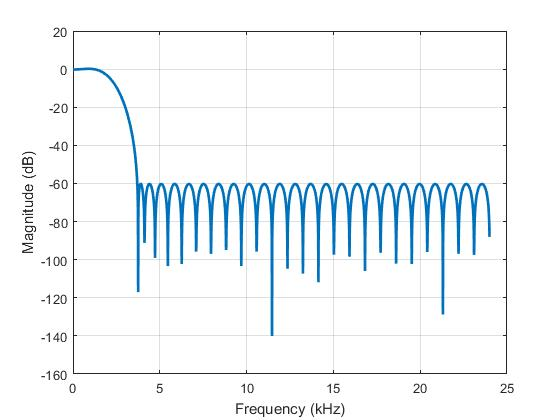
\includegraphics[width=0.8\textwidth]{./img1}
\caption{Filter magnitude response}
\label{f:fig1}
\end{figure}

\subsection{Program - myfir}

Implementing the filter as a function in C required six inputs: input, filterCoeffs, output, delayLine, nx, and nh. Input and output were pointers for the data being passed into the filter and being returned from the filter, respectively. FilterCoeffs was a pointer to the array of filter coefficients. DelayLine was a pointer to an array of past inputs. Nx was the number of data points being passed through the filter each function call and nh was the number of filter coefficients.

DelayLine was updated at the start of every function call such that the nx new data were placed at the end of DelayLine, which still contained the previous (nh-1) data samples. Then, a nested for loop, Listing \ref{l:MAC}, was used to perform the convolution to generate the output. The signed 16-bit or Q0.15 filter coefficients and input samples (delayLine) were typecasted to signed 32-bit or Q1.30 and multiplied. The product was accumulated in a Q1.30 sum variable each time through the interior for loop, which ran for a number of iterations equal to the number of coefficients. The commented-out code in line six, was the MAC implementation using intrinsics. After completing all MACs, the Q1.30 sum variable was bit-shifted righ 15 bits and typecasted to a signed 16-bit integer to return a Q0.15 form output. After storing the output, delayLine was updated to shift the (nh-1) samples at the end of the array to the front of the array so the new nx samples could be loaded in the rear when myfir( ) was called next. Also, note the indices of filterCoeffs and delayLine: The filterCoeffs elements were called from front-to-back and the delayLine elements were called back-to-front. This corresponds to the flipping of the impulse response as discussed in Background.

Listing \ref{l:myfir} shows the for loop and function call used to apply myfir( ) to single input samples. Special care was taken when passing inputTestVector and out1 to the function because the location of input and output data from previous function calls had to be accounted for. Otherwise, every time myfir( ) was called the same input data would be filtered and the the output would be stored in the same location.

\begin{lstlisting}[caption={Snippet of code to perform convolution of filter and input data}, label=l:MAC]
for (i = 0; i < nx; i++)
{
	for (j = 0; j < nh; j++)
	{
		sum += ((int32_t)(filterCoeffs[j]) * (int32_t)(delayLine[i + nh - 1 -j]));
		// sum = _smac(sum, filterCoeffs[j], delayLine[i + nh - 1 - j]);
	}

	output[i] = (int16_t)(sum >> 15);
	sum = 0;
}
\end{lstlisting}

\begin{lstlisting}[caption={Snippet of code the myfir( ) funtion call}, label=l:myfir]
 for(i = 0; i < inLen; i += myNX)
{
	myfir(&inputTestVector[i], h53, &out1[i], delayLine1, myNX, myNH);
}
\end{lstlisting}

\subsection{Program - Audio Filtering}

For the project demonstration, audio was played into the ezDSP, filtered and played back. To accomplish the audio loop, code was borrowed from the \textbf{aic3204} program. Listing \ref{l:audio} show the code used to read, filter and write the audio data. As there was left and right data, myfir( ) was called twice and two separate delay lines were used. 

\begin{lstlisting}[caption={Snippet of code to read, filter and write data}, label=l:audio]
    for ( sec = 0 ; sec < 10 ; sec++ )
    {
        for ( msec = 0 ; msec < 1000 ; msec++ )
        {
            for ( sample = 0 ; sample < 48 ; sample++ )
            {
                /* Read 16-bit left channel Data */
                EZDSP5535_I2S_readLeft(&data1);
                
                /* Read 16-bit right channel Data */
                EZDSP5535_I2S_readRight(&data2);
                
                /* Filter left channel Data */
                myfir((int16_t *)&data1, h53, (int16_t *)&out1, delayLine1, 1, 54);

                /* Filter right channel Data */
                myfir((int16_t *)&data2, h53, (int16_t *)&out2, delayLine2, 1, 54);

                /* Write 16-bit left channel Data */
                EZDSP5535_I2S_writeLeft(out1);
                
                /* Write 16-bit right channel Data */
                EZDSP5535_I2S_writeRight(out2);
            }
        }
    }
\end{lstlisting}

\section{Results}

\subsection{MATLAB v Embedded Implementation}

If implemented correctly, the embedded filter should have produced very similar output compared to the MATLAB generated output, with some error from rounding. Figure \ref{f:fig2} shows the graph of the output (top) of the embedded C and MATLAB implementations. As shown, the outputs are nearly identical. The bottom graph shows the absolute difference between the two outputs. It appeared that the greatest difference occurred at the peaks and valleys of the sinusoid. 

As measure of similarity, the mean-squared error (MSE) between the C and MATLAB outputs was calculated. For the 240 samples recorded, a MSE of \(2.95*10^{-8}\) was calculated. Again, the embedded C implementation was nearly identical to the theoretical MATLAB filter output.

\begin{figure}[h]
\centering
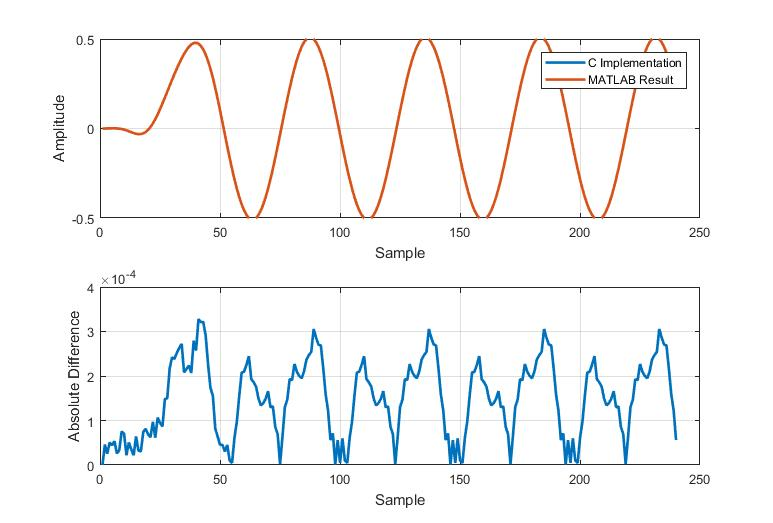
\includegraphics[width=0.8\textwidth]{./img2}
\caption{MATLAB and embedded filter output, Difference graph}
\label{f:fig2}
\end{figure}

\subsection{Filter Delay}

Theoretically, the delay of a FIR filter is equal to \(\frac{M}{2}\). The designed filter was 53rd order; hence, the delay was expected to be 26.5 samples. To determine the actual delay, a 1,000 Hz sinusoid of one period in length was generated in MATLAB. The sinusoid was drug across the embedded filter output and at each increment the MSE was calculated. The sample number that corresponding to a minimum MSE was the number of delayed samples. Sample 26 and 27 were about equivalent and were the minimum, so it was concluded that the delay was 26.5 samples.

\subsection{Cycle Efficiency}

For a filter to be a real-time filter, the filter must be able to perform all MACs required on the input data and return the output before the next sample is obtained. For this project, the ezDSP operated at 100 MHz and the codec sampling rate was 48 MHz; therefore, the filter had 2,083 cycles per sample to perform all operations.

The implementation of the filter with standard code, as discussed in Program - myfir, and no optimization required 2,623 cycles. At that number of cycles, the filter would not be able to operate in real-time because it required more the 2,083 cycles per sample. Using code composer compiler optimization improved the cycle efficiency to 2130, 2125, 568 and 565 for level 0, 1, 2, and 3 optimization, respectively. At optimization levels 2 and 3, the filter would have been able to operate in real time.

The use of intrinsics, as discussed in Program - myfir, was also used to try and reduce the cycle requirements. With no optimization and using intrinsics, the filter used 2,787 cycles per sample. The cycle requirements increased with intrinsics, which was unexpected at level 0 and 1 optimization the intrinsics reduced cycle use to 2022 and 2019, respectively, which would have been able to run in real-time. However, at optimizationg levels 2 and 3 the intrinsic code was less efficient than standard code at 573 and 568 cycles per sample, respectively. It is unclear why the intrinsic decreased cycle efficiency.

The 565 cycles per sample was best cycle efficiency achieved. It was achieved with all critical pieces of memory in dual-access RAM. Memory was then placed in single-access RAM to observe the effect of memory allocation. With all memory allocated to single-access RAM, the number of cycles increased minimally to 571. The impact of memory type was less significant than expected. 

The relationship between the number of coefficients and the cycle requirements was determined by collecting data from 60th, 70th, 80th, 90th, and 100th order filters at level 3 optimization. The results were 628, 718, 808, 898, and 988, respectively. Based on the data, the relationship was linear and equal to \(9*M + 88\). Based on this relationship, the maximum order filter that could be used in a real-time application was a 221st order filter. Such a filter was designed with fdatool and implemented; the cycle requirement was 2,077 cycles per sample, which was within the real-time bounds. 

The CPU requirements of the filter were not measured due to problems using the system analyzer tools.

\subsection{Demonstration}

The 53rd order filter was used to filter the audio samples. As mentioned, the presence of left and right audio sample required two filter operations per sample. Hence, to operate in real-time the filter had to have cycle efficiency less than 1,041 cycles per sample. Additionally, the cycles to read and write audio had to be accounted for so a cycle efficiency of 900 cycles per sample would be the approximate bound. The 53rd order filter at 565 cycles per sample was clearly under that bound. The loop to read, filter and write required 1,248 cycles. The filtered audio output was muffled and sounded distant. There was a distinct lack of sharpness to sounds that would likely be attributed to the high frequency components that are capable of producing rapid changes in sound.

\section{Summary}

The purpose of this project was to design an FIR filter and implement the filter in a real-time embedded system application. The project demonstrated the importance of cycle efficiency when operating in real-time. Any filter can be designed in MATLAB but trade-offs of time and quality must be made when implementing filters in a practical application. The real-time bound for this project was 2,083 cycles per sample and the filter implemented required 565 cycles at max optimization.

\pagebreak

\section{Appendix}

\begin{lstlisting}[caption={main}, label=l:main]
/*
 * main.c
 */

#include "stdint.h"
#include "stdio.h"
#include "string.h"
#include "testVector.h"
#include "ezdsp5535.h"
#include "ezdsp5535_gpio.h"
#include "ezdsp5535_i2c.h"

#define myNH 		  54	// # of filter coefficients
#define myNX 		   1	// # of samples evaluated per function call
#define inLen		 240	// # of total input samples

/* Coefficient array (length = 54) of a 53rd order FIR filter */
const int16_t h53[] =
{
        24,     17,     17,     11,     -5,    -32,    -72,   -123,   -184,   -249,   -309,   -354,   -374,   -354,   -286,   -159,
        32,    287,    601,    962,   1354,   1755,   2141,   2489,   2773,   2975,   3080,   3080,   2975,   2773,   2489,   2141,
      1755,   1354,    962,    601,    287,     32,   -159,   -286,   -354,   -374,   -354,   -309,   -249,   -184,   -123,    -72,
       -32,     -5,     11,     17,     17,     24
};

int16_t out1[inLen];

int16_t delayLine1[myNH + myNX - 1];
int16_t delayLine2[myNH + myNX - 1];

extern Int16 aic3204_loop_linein( );

extern void myfir(const int16_t* input, const int16_t* filterCoeffs, int16_t* output,
		int16_t* delayLine, uint16_t  nx, uint16_t  nh);

/*
 * main -
 */

int main(void)
{
    /* Initialize BSL */
    EZDSP5535_init( );

    /* Initialize I2C */
    EZDSP5535_I2C_init( );

	static uint16_t i;

	/* Inialize output and delay line arrays to zeros */
	memset( out1, 0, sizeof( out1 ) );
	memset( delayLine1, 0, sizeof( delayLine1 ) );
	memset( delayLine1, 0, sizeof( delayLine1 ) );

	while(1)
	{

//		for(i = 0; i < inLen; i += myNX)
//		{
//			myfir(&inputTestVector[i], h53, &out1[i], delayLine1, myNX, myNH);
//		}

		aic3204_loop_linein( );

		/* Clear out1 and delayLine1 */
		memset( out1, 0, sizeof( out1 ) );
		memset( delayLine2, 0, sizeof( delayLine2 ) );
		memset( delayLine2, 0, sizeof( delayLine2 ) );
	}

	return 0;
}
\end{lstlisting}

\pagebreak

\begin{lstlisting}[caption={aic3204 audio loop}, label=l:aic3204]
#include "stdio.h"
#include "stdint.h"
#include "ezdsp5535.h"
#include "ezdsp5535_i2s.h"
#include "csl_i2s.h"

extern Int16 AIC3204_rset( Uint16 regnum, Uint16 regval);

extern void myfir(const int16_t* input, const int16_t* filterCoeffs, int16_t* output,
		int16_t* delayLine, uint16_t  nx, uint16_t  nh);

extern const int16_t h53[];

extern int16_t delayLine1[54];

extern int16_t delayLine2[54];

/*
 *  AIC3204 Loop
 * 
 *      Loops audio from LINE IN to LINE OUT
 */
Int16 aic3204_loop_linein( )
{
    Int16 sec, msec;
    Int16 sample, data1, data2, out1, out2;
     
    /* Configure AIC3204 */
    AIC3204_rset( 0,  0x00 );  // Select page 0
    AIC3204_rset( 1,  0x01 );  // Reset codec
    EZDSP5535_waitusec(1000);  // Wait 1ms after reset
    AIC3204_rset( 0,  0x01 );  // Select page 1
    AIC3204_rset( 1,  0x08 );  // Disable crude AVDD generation from DVDD
    AIC3204_rset( 2,  0x01 );  // Enable Analog Blocks, use LDO power
    AIC3204_rset( 123,0x05 );  // Force reference to power up in 40ms
    EZDSP5535_waitusec(50000); // Wait at least 40ms
    AIC3204_rset( 0,  0x00 );  // Select page 0
    
    /* PLL and Clocks config and Power Up  */
    AIC3204_rset( 27, 0x0d );  // BCLK and WCLK are set as o/p; AIC3204(Master)
    AIC3204_rset( 28, 0x00 );  // Data ofset = 0
    AIC3204_rset( 4,  0x03 );  // PLL setting: PLLCLK <- MCLK, CODEC_CLKIN <-PLL CLK
    AIC3204_rset( 6,  0x07 );  // PLL setting: J=7
    AIC3204_rset( 7,  0x06 );  // PLL setting: HI_BYTE(D=1680)
    AIC3204_rset( 8,  0x90 );  // PLL setting: LO_BYTE(D=1680)
    AIC3204_rset( 30, 0x88 );  // For 32 bit clocks per frame in Master mode ONLY
                               // BCLK=DAC_CLK/N =(12288000/8) = 1.536MHz = 32*fs
    AIC3204_rset( 5,  0x91 );  // PLL setting: Power up PLL, P=1 and R=1
    EZDSP5535_waitusec(10000); // Wait for PLL to come up    
    AIC3204_rset( 13, 0x00 );  // Hi_Byte(DOSR) for DOSR = 128 decimal or 0x0080 DAC oversamppling
    AIC3204_rset( 14, 0x80 );  // Lo_Byte(DOSR) for DOSR = 128 decimal or 0x0080
    AIC3204_rset( 20, 0x80 );  // AOSR for AOSR = 128 decimal or 0x0080 for decimation filters 1 to 6
    AIC3204_rset( 11, 0x82 );  // Power up NDAC and set NDAC value to 2
    AIC3204_rset( 12, 0x87 );  // Power up MDAC and set MDAC value to 7
    AIC3204_rset( 18, 0x87 );  // Power up NADC and set NADC value to 7
    AIC3204_rset( 19, 0x82 );  // Power up MADC and set MADC value to 2
    
    /* DAC ROUTING and Power Up */
    AIC3204_rset( 0,  0x01 );  // Select page 1
    AIC3204_rset( 12, 0x08 );  // LDAC AFIR routed to HPL
    AIC3204_rset( 13, 0x08 );  // RDAC AFIR routed to HPR
    AIC3204_rset( 0,  0x00 );  // Select page 0
    AIC3204_rset( 64, 0x02 );  // Left vol=right vol
    AIC3204_rset( 65, 0x00 );  // Left DAC gain to 0dB VOL; Right tracks Left
    AIC3204_rset( 63, 0xd4 );  // Power up left,right data paths and set channel
    AIC3204_rset( 0,  0x01 );  // Select page 1
    AIC3204_rset( 16, 0x00 );  // Unmute HPL , 0dB gain
    AIC3204_rset( 17, 0x00 );  // Unmute HPR , 0dB gain
    AIC3204_rset( 9 , 0x30 );  // Power up HPL,HPR
    EZDSP5535_waitusec(100 );  // Wait
    
    /* ADC ROUTING and Power Up */
    AIC3204_rset( 0,  0x01 );  // Select page 1
    AIC3204_rset( 52, 0x30 );  // STEREO 1 Jack
                               // IN2_L to LADC_P through 40 kohm
    AIC3204_rset( 55, 0x30 );  // IN2_R to RADC_P through 40 kohmm
    AIC3204_rset( 54, 0x03 );  // CM_1 (common mode) to LADC_M through 40 kohm
    AIC3204_rset( 57, 0xc0 );  // CM_1 (common mode) to RADC_M through 40 kohm
    AIC3204_rset( 59, 0x00 );  // MIC_PGA_L unmute
    AIC3204_rset( 60, 0x00 );  // MIC_PGA_R unmute
    AIC3204_rset( 0,  0x00 );  // Select page 0
    AIC3204_rset( 81, 0xc0 );  // Powerup Left and Right ADC
    AIC3204_rset( 82, 0x00 );  // Unmute Left and Right ADC
    AIC3204_rset( 0,  0x00 );  // Select page 0 
    EZDSP5535_waitusec(100 );  // Wait
    
    /* Initialize I2S */
    EZDSP5535_I2S_init();
     
    /* Play Loop for 10 seconds */
    for ( sec = 0 ; sec < 10 ; sec++ )
    {
        for ( msec = 0 ; msec < 1000 ; msec++ )
        {
            for ( sample = 0 ; sample < 48 ; sample++ )
            {
                /* Read 16-bit left channel Data */
                EZDSP5535_I2S_readLeft(&data1);
                
                /* Read 16-bit right channel Data */
                EZDSP5535_I2S_readRight(&data2);
                
                /* Filter left channel Data */
                myfir((int16_t *)&data1, h53, (int16_t *)&out1, delayLine1, 1, 54);

                /* Filter right channel Data */
                myfir((int16_t *)&data2, h53, (int16_t *)&out2, delayLine2, 1, 54);

                /* Write 16-bit left channel Data */
                EZDSP5535_I2S_writeLeft(out1);
                
                /* Write 16-bit right channel Data */
                EZDSP5535_I2S_writeRight(out2);
            }
        }
    }
    EZDSP5535_I2S_close();    // Disble I2S
    AIC3204_rset( 1, 0x01 );  // Reset codec
    
    return 0;
}

\end{lstlisting}

\pagebreak

\begin{lstlisting}[caption={myfir}, label=l:myfir]
/*
// *****************************************************************************
// *****************************************************************************
// **
// ** File Name: myfir.c
// **
// ** Author: David McCreight
// **
// ** Description: 
// **              
// **
// *****************************************************************************
// *****************************************************************************
*/

/*******************************************************************************
****                            I N C L U D E S 
*******************************************************************************/

#include "stdint.h"
#include "stdio.h"

/*******************************************************************************
****                         D E F I N I T I O N S
*******************************************************************************/

/*******************************************************************************
****                   S T A T I C   V A R I A B L E S  
*******************************************************************************/

/*******************************************************************************
****                    G L O B A L   V A R I A B L E S  
*******************************************************************************/

/*******************************************************************************
****          F U N C T I O N   D E F I N I T I O N S 
*******************************************************************************/
void myfir(const int16_t* input,
             const int16_t* filterCoeffs,
			 int16_t* output,
			 int16_t* delayLine,
			 uint16_t  nx,
			 uint16_t  nh)
{
    
    uint16_t i;
    uint16_t j;
    long sum = 0;
	
    /*
     * Assumes delayLine length is nh - 1 + nx
     */

    // copy input samples to the delay line
    for (i = 0; i < nx; i++)
    {
        delayLine[i + nh - 1] = input[i];
    }

	for (i = 0; i < nx; i++)
	{
		for (j = 0; j < nh; j++)
		{
			sum += ((int32_t)(filterCoeffs[j]) * (int32_t)(delayLine[i + nh - 1 -j]));
//			sum = _smac(sum, filterCoeffs[j], delayLine[i + nh - 1 - j]);
		}

		output[i] = (int16_t)(sum >> 15);
		sum = 0;
	}
		
    // Update delay line for next function call
	for (i = 0; i < (nh - 1); i++)
	{
		delayLine[i] = delayLine[nx + i];
	}
}

/*******************************************************************************
 ****                        E N D   O F   F I L E
 *******************************************************************************/
\end{lstlisting}

\pagebreak

\begin{lstlisting}[caption={MATLAB analysis code}, label=l:ml]
testVector = 2 * ParseGenericDataFile( 'int16','testVector.dat' ) / 32786;
ccsOut = 2 * ParseGenericDataFile( 'int16', 'outFIR1smp.dat' ) / 32786;
matlabOut = filter( h53, 1, input(1,1:240)');

T = 1/48;
fs = 48000;
t = 0:1:48;
pureSine = 0.5 * sin( 2*pi*1000/fs*t )';

[ h1, w1 ] = freqz( h53, 1, 2048,fs);

mseTest = zeros( 100, 1 );
diff = zeros( 240, 1 );

for m = 1:100
    mseTest( m, 1 ) = immse( pureSine, ccsOut(m:(m+48), 1 ) );
end

for k = 1:240
   diff( k, 1 ) = abs( matlabOut( k, 1 ) - ccsOut( k, 1 ) );
end

mse1 = immse( ccsOut, matlabOut )

figure(1)
subplot( 2, 1, 1 )
plot( 1:1:240, ccsOut, 1:1:240, matlabOut, 'Linewidth', 2 )
grid on
legend( "C Implementation", "MATLAB Result" )
xlabel( "Sample" )
ylabel( "Amplitude" )
subplot( 2, 1, 2 )
plot(diff, 'Linewidth', 2 )
grid on
xlabel( "Sample" )
ylabel( "Absolute Difference" )

figure(2)
plot( w1/1000, 20*log10(abs(h1)), 'Linewidth', 2 );
grid on
xlabel( "Frequency (kHz)" )
ylabel( "Magnitude (dB)" )
\end{lstlisting}

\end{document}



